\documentclass{article}
\usepackage[T1]{fontenc}
\usepackage[margin=1in, papersize={9in, 12in}]{geometry}
\usepackage{fontspec, nopageno, xltxtra, xunicode}
\usepackage{lilyglyphs}
\usepackage{tikz}
\usetikzlibrary{arrows}
\usetikzlibrary{shapes}
\parindent=0pt
\parskip=12pt
\setmainfont{Adobe Garamond Pro}
\usepackage{booktabs}
\usepackage[normalem]{ulem}
\useunder{\uline}{\ul}{}
\begin{document}

\begin{center}
  {\Huge Performance Notes }
\end{center}

{\huge Temporality}

The score of \textit{Un Jour à Rouen} is notated proportionally.
Beams indicate duration of sound, and notes that share a beam should be played
as legato as possible. In fact, except for moment of pizzicato and col legno
battuto, the entirety of the piece should be played in this way.
\begin{center}
  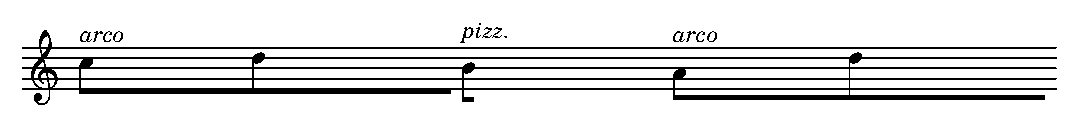
\includegraphics[scale=.8]{./duration2.pdf}
\end{center}
Each system lasts for 16 seconds, as denoted by the increasing time count
at the right edge of each system.  A tick mark on each staff indicates
the halfway point (8 seconds).

While for most of the piece, each player is following their own part score, there
are moments throughout where one or more players must play in unison. These are
outlined in grey, as shown below, and can provide a method of synchronizing the
ensemble.

\begin{center}
  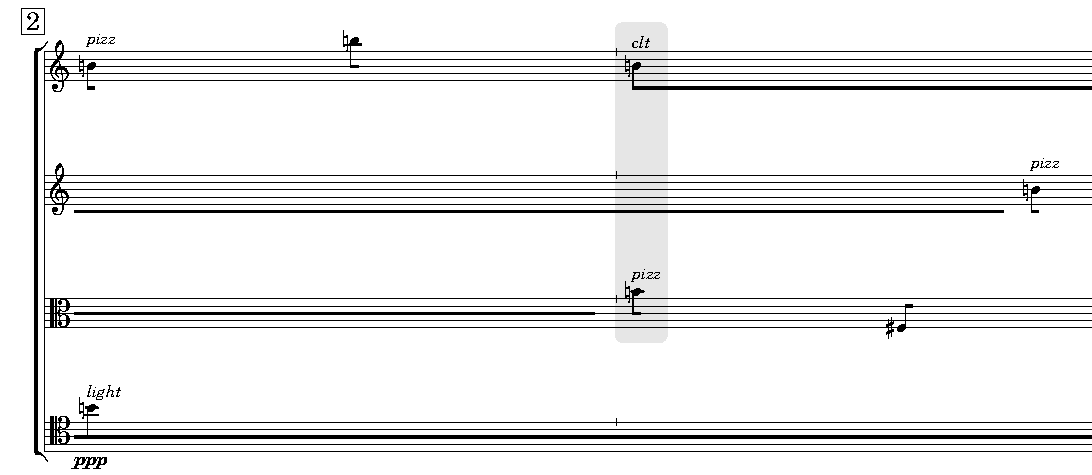
\includegraphics[scale=.8]{./score-page1-crop.pdf}
\end{center}

{\large Keeping Time}

The ensemble is welcome to set a stopwatch on a phone or tablet, positioned so
that the quartet can see it; or each use their own; or simply internalize the
passage of timing, using the moments described below to remain synchronized.
I leave this it to the performers to keep time in whatever manner they prefer.
\vspace{2em}

{\huge Notation}

{\large Dynamics}

Each instrument follows a linear dynamic shape from \textbf{\textit{niente}} to \lilyDynamics{f}
and back to \textit{\textbf{niente}}. Each notated increase is only a single dynamic
degree (i.e. \lilyDynamics{pp} to \lilyDynamics{p}, or \lilyDynamics{mf} to \lilyDynamics{mp}).
After their original statement, dynamics are restated, as necessary, in the first
system of each page, and at the beginning of hairpins.

At some points, instruments may be playing at greatly different dynamic levels.
In these instances, every voice should be heard, with the notated dynamics
understood as relative to one another, rather than absolute. Adjustments should be
made, to whatever degree possible, while still maintaining the overall shape of
each individual voice. Where adjustments must be made between the players, I would
prefer that louder dynamics be softened, rather than softer dynamics increased.

\pagebreak
% \vspace{2em}


{\large Techniques}

In \textit{Un Jour à Rouen}, there are 7 notated methods of producing sound from the instruments:
\begin{itemize}
  \item 4 degrees of \textit{arco}
  \item \textit{col legno tratto}
  \item \textit{col legno battuto}
  \item \textit{pizzicato}
\end{itemize}

These are notated in the score as

\begin{center}
  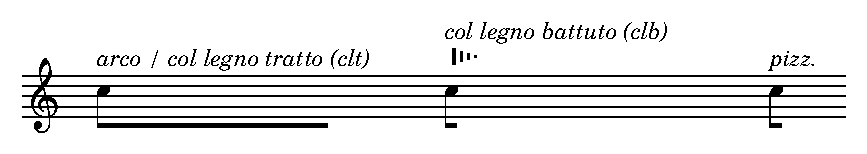
\includegraphics[scale=.8]{./attacks2.pdf}
\end{center}

and are defined as follows:

The degrees of \textit{arco} are notated as \textit{light}, \textit{ord}, \textit{mid} and \textit{heavy}:

\begin{itemize}
  \item \textit{light} - \textit{flautando} bow pressure, but with the left hand applying normal pressure on the string
  \item \textit{ord} - your ordinary, everyday, garden variety bow pressure
  \item \textit{mid} - somewhere between \textit{ord} and \textit{heavy}
  \item \textit{heavy} - a bit of overpressure, such that the sound is slightly distorted, but still predominantly pitched. This might be more easily and acceptably achieved via a slight overpressure combined with a drastic slowing of the bow, rather than a large adjustment in bow pressure.
    % ([Modern Cello Techniques | Pressure Techniques Overview](http://www.moderncellotechniques.com/bow-techniques/pressure-techniques/pressure-techniques-overview/))
\end{itemize}

\textit{pizzicato} - normal pizzicato

\textit{col legno battuto} -  as indicated by the notation, allow the wood of
the bow to bounce a few times in quick succession before coming to rest on
the string. This is indicated by \textit{clb} in the score.

\textit{col legno tratto} - notated as \textit{clt} in the score, this is
meant to produce a thinner, \textit{lontano} quality of sound.

Each player should perform each technique at a different point along the string.
These points are given in the table below

\begin{table}[h!]
  \begin{center}
    \label{tab:table1}
    \begin{tabular}{l|c|c|c|c|c|c|c} % <-- Alignments: 1st column left, 2nd middle and 3rd right, with vertical lines in between
      % \textbf{Value 1} & \textbf{Value 2} & \textbf{Value 3}\\
      % $\alpha$ & $\beta$ & $\gamma$ \\
      \space              & \textit{clt}   & \textit{light} & \textit{ord}   & \textit{mid}  & \textit{heavy} & \textit{pizz}  & \textit{clb} \\
      \hline
      \textbf{Violin I}   & sul tasto (st)   & norm  & sul ponticello (sp)   & norm    & molto sul tasto (mst)  & norm  & molto sul ponticello (msp) \\
      \hline
      \textbf{Violin II}  & norm  & sp    & norm  & mst     & norm  & msp   & st  \\
      \hline
      \textbf{Viola}      & sp    & norm  & mst   & norm    & msp   & st    & norm \\
      \hline
      \textbf{'Cello}     & norm  & mst   & norm  & msp     & st    & norm  & st \\
      \hline
    \end{tabular}
  \end{center}
\end{table}

Where one degree of bow pressure is followed by another, the transition
should be made gradually, rather than suddenly. The notation of a changed
pressure indicates the point at which the player should arrive at this new
pressure, not when the transition should begin. To whatever degree is possible,
the transition to the new point along the string, in the table above, should be
made gradual as well, though priority should be given to the change in technique.

For the purposes of these transitions, \textit{col legno tratto} should also
be treated as \textit{arco}. To whatever extent possible, when transitioning
into or out of \textit{col legno tratto}, the player should rotate the
bow to create a smooth shift in sound.

Transitions to or from \textit{pizz} and \textit{col legno battuto}
will by necessity be immediate.



% \input{../_assets/preface-body-1.tex}
\break
{\large Accidentals}

\textit{Un Jour à Rouen} is notated in equal temperament.

In addition to the standard chromatic accidentals \hspace{.2em} \flat, \sharp, and \natural, the following accidentals are used:

\lilyGlyph[scale=1.5,raise=.5]{accidentals.sharp.slashslashslash.stemstem} \hspace{.2em} three quarters sharp

\lilyGlyph[scale=1.5,raise=.5]{accidentals.sharp.slashslash.stem} \hspace{.2em} one quarter sharp

\lilyGlyph[scale=1.5,raise=.5]{accidentals.mirroredflat} \hspace{.5em} one quarter flat

\lilyGlyph[scale=1.5,raise=.5]{accidentals.mirroredflat.flat} \hspace{.5em} three quarters flat

\lilyGlyph[scale=1.5,raise=.5]{accidentals.flat.arrowup} \hspace{.5em}
\lilyGlyph[scale=1.5,raise=.5]{accidentals.natural.arrowup} \hspace{.5em}
\lilyGlyph[scale=1.5,raise=.5]{accidentals.sharp.arrowup} \hspace{.5em} one 1/8 tone higher

\lilyGlyph[scale=1.5,raise=.5]{accidentals.flat.arrowdown} \hspace{.5em}
\lilyGlyph[scale=1.5,raise=.5]{accidentals.natural.arrowdown} \hspace{.5em}
\lilyGlyph[scale=1.5,raise=.5]{accidentals.sharp.arrowdown} \hspace{.5em} one 1/8 tone lower

These 1/8 tones do not need to be exactly tuned in every case. They function ultimately as a shading of a pitch, and thus should be
noticeably different from, but not necessarily exactly between, the chromatic pitch and its neighboring quarter tone.

Throughout, accidentals apply only to the note to which they are attached.

% \vspace{1em}
\vfill
\textsl{
Between 1892 and 1893, Claude Monet made a series of more than two dozen paintings
of the Rouen Cathedral, each capturing its façade at a different time of day and year.
Although the architecture of the cathedral fills each canvas, Monet's true subject was
the light; as it changed from day to day, hour to hour, and even minute to minute, in
the course of a single painting.
}

\textsl{
This piece uses four of these paintings, spanning a full day of light on Rouen
Cathedral, as its source material. Four lines begin from a single point and each
follow an identical harmonic development before re-converging on a single, but
different, point. Like the light in Monet's paintings, it is the ever-shifting
variations in bowing technique that gives each line its distinct timbre.
}

\end{document}
